\section{Matriz de tiempos de residencia}\label{met:matriz}

En la sección anterior se planteó el modelo multiclase con dispersión virtual. La principal diferencia con respecto a otros modelos multiclase estaba en la forma en que se calculaba la tasa de contagio; las \(n\) clases interactúan en \(m\) ambientes virtuales. Esta interacción está codificada por medio de la matriz de tiempos de residencia \( \mathbf{R} =\{r_{i,j}\}_{i \in 1 \dots n, j \in 1 \dots m}\), donde la entrada \(r_{ij}\) corresponde a la fracción del día que la clase \(i\) pasa en el ambiente \(j\).

El objetivo de este apartado es elegir las clases y ambientes a utilizar para estudiar el caso de Santiago, y estimar la matriz \(\mathbf{R}\) de tiempos de residencia asociada. Es importante notar que esta matriz será variable en el tiempo, puesto que las diferentes medidas de mitigación (cierre de instituciones educativas, cuarentenas) implementadas por el gobierno de Chile ([link]) han cambiado significativamente el modo de vida en la ciudad.  

Se comienza eligiendo las clases y ambientes a utilizar. Posteriormente, se describirá la metodología para la obtención de una matriz de tiempos de residencia \(\mathbf{R}^0\) correspondiente a la ciudad de Santiago en condiciones normales. Finalmente se describirá la metodología para modificar esta matriz, con el fin de reflejar las variaciones en el comportamiento de la población a lo largo del desarrollo de la pandemia, lo que da lugar a la matriz \(\mathbf{R}(t)\) definitiva.


\subsection{Elección de clases y ambientes}

Hay varios criterios a considerar a la hora de elegir las clases y los ambientes. En primer lugar, es ampliamente conocido \cite{} que la edad es un factor importante en el efecto de la enfermedad en una persona; el Covid19 afecta con más intensidad a los adultos mayores. Varios estudios \cite{} % alguno internacional 
\cite{Mena2021}\cite{Bennett2021} han mostrado que la pandemia ha afectado más fuertemente a los niveles socioeconómicos o comunas más pobres y lo asocian, entre otras cosas, a la dificultad de ellos de acatar las cuarentenas. Se ha mencionado también el sexo como una variable a tener en cuenta \cite{}, y la Encuesta Origen Destino muestra diferencias en el uso del tiempo entre hombres y mujeres \cite{Jara-Diaz2013}.

Los datos disponibles han de ser considerados también. La Encuesta Origen Destino, por un lado, posee datos muy granulares; es posible conocer para un individuo su sexo, zona censal y comuna donde reside, edad e ingreso familiar. Más aún, los distintos propósitos de los viajes realizados (regreso al hogar, al trabajo, escuela, compras, transporte público, bicicleta, entre otros) entregan varios ambientes donde ese individuo pasa su tiempo. 

Por otro lado, las demás fuentes de datos no poseen tanta información. El Uso de infraestructura de telecomunicaciones permite conocer cómo ha cambiado la movilidad de entrada o salida a cada zona censal/comuna, pero no distingue entre las actividades que realizan las personas mientras se mueven por la ciudad. Los Informes de Movilidad Local sobre Covid19 de Google permiten distinguir distintas actividades, pero no permiten separar por comuna.

Las series de tiempos de Datos-COVID19 presentan dificultades similares. Están desagregadas por edad, sexo o comuna, pero no por los tres criterios simultáneamente.

Puesto que se desea considerar el efecto de las cuarentenas en el uso del tiempo de las personas a lo largo de la pandemia, sabiendo la importancia que juega en las diferencias entre las distintas comunas, se decide usar los datos de Uso de infraestructura de telecomunicaciones. Esto lleva a desechar la información de los distintos ambientes; se sabe que hay más o menos movilidad fuera del hogar, pero no se sabe exactamente en qué actividad. El trabajo considera, por tanto, solo \(m = 2\) ambientes: \texttt{hogar} y \texttt{exterior}. Siguiendo a \cite{Ferguson2020}, el número de contagios en el hogar es aproximadamente de 1/3, por lo que, ya que se fijó \(\beta_{\text{hogar}} = 1\), se supondrá que \(\beta_{\text{exterior}} \approx 2\).

Los datos elegidos permiten utilizar la información a nivel de zona censal, pero los datos epidemiológicos no son tan granulares, por lo que es más factible distinguir por comuna. Los datos epidemiológicos están disponibles a este nivel también, por lo que es una buena posibilidad. Eso, sin embargo, plantearía un sistema con unas 50 clases, lo que para 4 compartimientos da unas 200 variables. Es posible, aunque agrega más carga computacional y dificulta el análisis posterior. Se decide, por simplicidad, reducir el análisis a \(n = 5\) categorías socioeconómicos, las mismas propuestas por \cite{SEREMIRM2019}, que surgen tras ordenar las comunas por IPS. Pueden verse en la Tabla \ref{table:ips-categ}.

Ante la falta de la información adecuadamente desagregada para edad y sexo, se decide abandonar estos criterios.

% Agregar población según CENSO 
\begin{table}[h!]
\centering
\begin{tabular}{|c c c c|} 
 \hline
 \textbf{Prioridad Social} & \textbf{IPS mínimo} & \textbf{IPS máximo} & \textbf{Ejemplos} \\ [0.5ex] 
 \hline
 Alta & 78.24 & 83.03 & La Pintana, Lo Espejo\\ 
 Media Alta & 73.84 & 77.39 & San Bernardo, El Bosque\\
 Media Baja & 65.05 & 71.36 & La Cisterna, Quinta Normal\\
 Baja & 53.34 & 64.37 & Santiago, Providencia\\
 Sin Prioridad & 6.26 & 37.36 & Las Condes, Lo Barnechea\\ [1ex] 
 \hline
\end{tabular}
\caption{Categorías socioeconómicas de IPS dadas por \cite{SEREMIRM2019}.}
\label{table:ips-categ}
\end{table}

\subsection{Matriz de Santiago en condiciones normales} 

% Acerca de los propósitos de viajes 
% Los propósitos son los siguientes:
% Al trabajo
% Por trabajo
% Al estudio
% Por estudio
% De salud
% Visitar a alguien
% Volver a casa
% Buscar o Dejar a alguien
% Comer o Tomar algo
% Buscar o dejar algo
% De compras
% Trámites
% Recreación
% Otra actividad 
En \cite{Munizaga2011} se propone un método para obtener información acerca del uso del tiempo de una persona a partir de los tiempos de inicio y fin de sus viajes, contenidos en la Encuesta Origen-Destino, y el propósito declarado de este. Para esto supone que el primer viaje comienza desde el hogar (esto puede verificarse revisando que calcen la zona de origen del viaje con la del hogar). Luego, a cada período de tiempo entre dos viajes consecutivos es asignado a la actividad declarada como propósito en el viaje anterior. La Figura \ref{img:ciclo-viajes} es un diagrama de este proceso. El Algoritmo \ref{alg:timematrix} explica el proceso en detalle de manera general, agregando además ambientes para los distintos modos de transporte. La matriz obtenida usando este algoritmo se denota \(\mathbf{R}_0\). La matriz variable en el tiempo será construida a partir de esta en la siguiente subsección.
% Insertar el algoritmo para esto, traducir 

\begin{figure}[H]
\centering
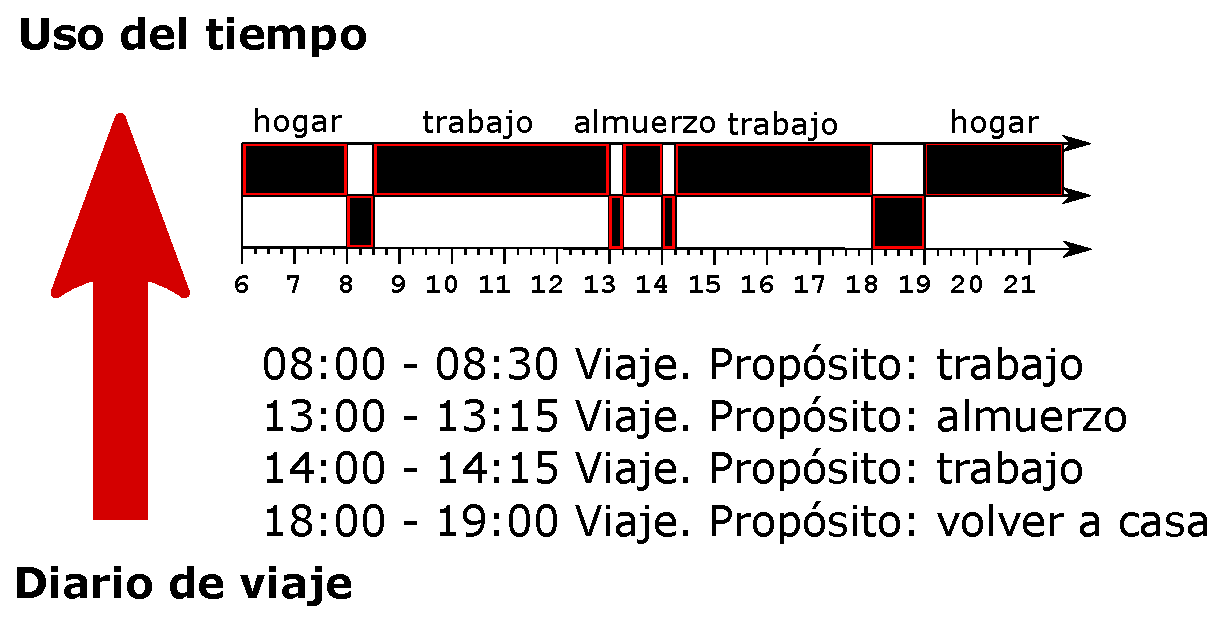
\includegraphics[width=.6\linewidth]{img/metodologia/matrizPnormal/ciclo-viajes.eps}
\caption[Transformar propósitos de viaje en tiempo de actividad.]{Transformar propósitos de viaje en tiempo de actividad. Fuente: \cite{Munizaga2011}, traducción propia.}
\label{img:ciclo-viajes}
\end{figure}

\begin{algorithm}[H]
\SetAlgoLined

\KwIn{
Una lista de personas \(P\). Para cada \(p \in P\), una lista \(V_p\) de todos los viajes hechos por \(p\), ordenados del primero al último. Para un viaje \(v\) es posible obtener \(t_0, t_f\) tiempos de inicio y fin, \(\mathtt{modo}\) de transporte y \(\mathtt{propósito}\) del viaje.
Dos funciones \( \mathcal{J}_{\mathtt{m}}: \mathtt{modo} \mapsto j\) y \(\mathcal{J}_{\mathtt{p}}: \mathtt{propósito} \mapsto j\) que asocian cada \texttt{modo} de transporte (bus, auto, etc) y cada \texttt{propósito} de viaje (al trabajo, de compras, etc) a un ambiente \(j \in \{1, \dots, m\}\) (trabajo, compras, transporte público, etc). Un ambiente por defecto \(j_0\) (hogar), donde las personas sin viajes pasan su tiempo, y donde las personas comienzan su primer viaje. Una función \(\mathcal{C}: p \in P \mapsto i\) que asigne a cada persona \(p\) una clase \(i \in \{1, \dots, n\}\). Tiempos de inicio \(T_0\) y fin \(T_f\) del intervalo de tiempo total considerado.
}

\KwResult{Una matriz de tiempos de residencia \(R = (r_{ij})_{i = 1 \dots n, j = 1 \dots m}\) donde \(r_{ij}\) es la fracción del tiempo que la clase \(i\) pasa en el ambiente \(j\). Solo considera personas sin viajes inválidos.}

%Elegir un grafo $G$ conexo y una matriz $R$. 

Definir la matriz auxiliar \(C = (c_{ij})_{i = 1 \dots n, j = 1 \dots m}\). \(c_{ij}\) guardará el tiempo total que las personas de la clase \(i\) pasan en el ambiente \(j\). Se inicializa en \(0\)\;

Definir \(T = T_f - T_0\) el tiempo total considerado.

Definir \(N_i \gets 0\) para cada \({i \in 1 \dots n}\) para contar el total de personas en cada clase. 

\ForAll{\(p \in P\)}{
    Guardar en \(i\) el valor \(\mathcal{C}(p)\), la clase de \(p\)\; %\tcc*[r]{class of person \(p\)} \;

    \uIf{La persona \(p\) no tiene viajes, \(V_p = \varnothing\)}{
        Se supone que \(p\) pasa todo su tiempo en el ambiente \(j_0\) por defecto. \(c_{i,j_0} \gets c_{i,j_0} + T\)\; 
        
        Contabilizar una persona válida. \(N_i \gets N_i + 1\)\;
    }
    \uElseIf{\(V_p\) tiene información faltante (\(\mathtt{propósito}, \mathtt{modo}, t_0\) or \(t_f\) de algún \(v \in V_p\) no está definido)}{
        \(p\) no es una persona válida y no es considerada en la matriz final\;
    }
    \Else{
        \(j\_\mathtt{anterior} \gets j_0 \). Ambiente donde terminó el viaje anterior. Comienza en \(j_0\)\;
        \(t_f\_\mathtt{anterior} \gets T_0\). Hora de término del viaje anterior. Vale \(T_0\) por defecto\;
        \ForAll{viaje \(v \in V_p\)}{
            Obtener \(\mathtt{prop\'osito}, \mathtt{modo}, t_0\) y \(t_f\) asociados al viaje \(v\). Definir \(j_v \gets \mathcal{J}_\mathtt{m}(\mathtt{modo})\) el ambiente asociado al modo del viaje \(v\)\;
            
            Agregar el tiempo entre el viaje anterior y el viaje \(v\) al ambiente donde terminó el viaje anterior. \(c_{i, j\_\mathtt{anterior}} \gets c_{i, j\_\mathtt{anterior}} + t_s - t_f\_\mathtt{anterior}\)\;
            
            Agregar el tiempo del viaje \(v\) a su ambiente asociado. \(c_{i, j_v} \gets c_{i, j_v} + t_f - t_s\)\;
            
            Actualizar  \(j\_\mathtt{anterior} \gets \mathcal{J}_{\mathtt{p}}(\mathtt{prop\'osito})\). El próximo viaje comienza donde \(v\) terminó.
            
            Actualizar \(t_f\_\mathtt{anterior} \gets t_f\). 
        }
        
        Agregar el tiempo entre el último viaje y el tiempo final \(T_f\) \(v\) al ambiente donde terminó el último viaje. \(c_{i, j\_\mathtt{anterior}} \gets c_{i, j\_\mathtt{anterior}} + T_f - t_f\_\mathtt{anterior}\)\;
        
        Contabilizar a \(p\) como una persona válida. \(N_i \gets N_i + 1\)\;
    }
    
}

Calcular \(R\) a partir de \(C\) normalizando cada fila. \(r_{ij} \gets c_{ij} / T N_i\)\;

\caption{Tiempos de residencia a partir de una lista de viajes}
\label{alg:timematrix}
\end{algorithm}

% Creo que sería bueno agregar el pseudo código de la cuestión. Estoy segura de que yo tenía una versión bonita de esto.
% Para que sea replicable tengo que incluir todas las pequeñas decisiones... los casos usados y los no usados, todo eso. 

% Proceso de manera diferenciada a los no viajeros de los viajeros. Se asume que los primeros pasan todo su tiempo en el hogar. 

% Redirigir a la imeplementación en Matlab.


\subsection{Variaciones de la matriz a lo largo del tiempo} 

% Explicar los datos disponibles
Se usan los datos de movilidad obtenidos del Uso de infraestructura de telecomunicaciones, descritos en \ref{data:isci}. Los datos se obtienen del repositorio de Datos-COVID19, descrito en \ref{data:minciencia}, del Producto 82 específicamente. 
% Nos estoy segura de qué tanto detalle tengo que dar aquí, puedo ser muy específica y describir hasta las columnas involucradas. Tal vez como un anexo... 

Los datos se encuentran en dos archivos en formato \texttt{.csv}, correspondientes a la movilidad durante días de la semana laborables \texttt{ISCI\_weeks.csv} y a la movilidad de los fines de semana \texttt{ISCI\_weekends.csv}. Se usa el primero de estos. Los atributos incluyen la comuna de la Región Metropolitana con nombre \texttt{nom\_comuna} y código único territorial \texttt{comuna} a la que corresponde la medición, semana epidemiológica \texttt{semana} de la medición con fecha de inicio \texttt{fecha\_inicio} y fin \texttt{fecha\_termino}, y estimaciones de la variación de movilidad \texttt{var\_salidas}, que es un promedio entre \texttt{var\_salidas\_cota\_superior} y \texttt{var\_salidas\_cota\_inferior}. 

Se utiliza la información de \texttt{var\_salidas} (despreciando las cotas inferiores y superiores). Si llamamos \(m_i^0\) a la movilidad de referencia inicial para la comuna \(i\)-ésima (la cual es desconocida), y \(m_i^k\) a la movilidad de la comuna \(i\)-ésima en la semana \(k\)-ésima posterior a esa semana de referencia, entonces \texttt{var\_salidas} reporta los valores \(p_i^k\), donde 

\[
m_i^k = p_i^k m_i^0
\]

Un detalle a considerar es que necesario calcular la variación de movilidad para los distintos grupos socioeconómicos, puesto que solo la tenemos para las comunas. Si la población de la comuna \(i\)-ésima es \(N_i\), e \(I\) es un conjunto de comunas, estimamos la movilidad grupal como 
\[
m^k_I = \sum_{i \in I}m^k_i N_i
\]

Buscamos un parámetro \(p_I^k\) tal que 
\[
m_I^k = p_I^k m_I^0
\]

Bajo el supuesto \(m_i^0 := m^0\) para cada \(i\), entonces es fácil ver que

\[
p_I^k = \sum_{i \in I} p_i^k N_i
\]

Supondremos que la movilidad es constante a lo largo de la semana (incluyendo fines de semana). Se define una función \(\mathtt{semana}(t)\) que a un tiempo \(t\) le asocia la correspondiente semana. Suponemos además que el tiempo que cada clase pasa en el ambiente \texttt{exterior} varió de manera proporcional a la movilidad. Eso permite calcular la columna \texttt{exterior} de la matriz de tiempos de residencia para cada grupo socioeconómico \(I\) como

\[
r_{I, \text{exterior}}(t) = p_I^{\mathtt{semana}(t)} r_{I,\text{exterior}}^0
\]

%% Definir una variable para el nombre del ambiente fuera del hogar o exterior 



% Finalmente la matriz de tiempos de residencia que varía en el tiempo 

Finalmente, el tiempo que no se ocupa en el ambiente \texttt{exterior} se pasa en el ambiente \texttt{hogar}, por lo que 
\[
r_{I, \text{hogar}}(t) = 1 - r_{I,\text{hogar}}(t)
\]